\documentclass[border=6pt,tikz]{standalone}
\usepackage{tikz}
\usepackage{amsmath,amssymb}
\usetikzlibrary{arrows.meta,positioning,fit,backgrounds,calc,shapes.geometric,decorations.pathreplacing,patterns}
\definecolor{ink}{HTML}{1B2430}
\definecolor{muted}{HTML}{6B7785}
\definecolor{accent}{HTML}{2F6FB5}
\definecolor{accent2}{HTML}{C1611F}
\definecolor{good}{HTML}{2E7D5B}
\definecolor{soft}{HTML}{EDF2F7}
\definecolor{soft2}{HTML}{FBEDE2}
\definecolor{soft3}{HTML}{E6F0E9}
\tikzset{
  box/.style={draw=ink,line width=.7pt,rounded corners=2pt,fill=soft,inner sep=4pt,align=center,font=\sffamily\small},
  boxa/.style={box,fill=soft2},
  boxb/.style={box,fill=soft3},
  plain/.style={align=center,font=\sffamily\small,text=ink},
  tiny/.style={align=center,font=\sffamily\scriptsize,text=muted},
  ar/.style={-{Stealth[length=2.4mm]},draw=ink,line width=.7pt},
  arm/.style={-{Stealth[length=2.4mm]},draw=muted,line width=.6pt,dashed},
  nd/.style={circle,draw=ink,line width=.7pt,fill=white,minimum size=7mm,inner sep=0pt,font=\sffamily\scriptsize},
  ndf/.style={nd,fill=soft},
  ndt/.style={nd,fill=soft2},
}

\begin{document}
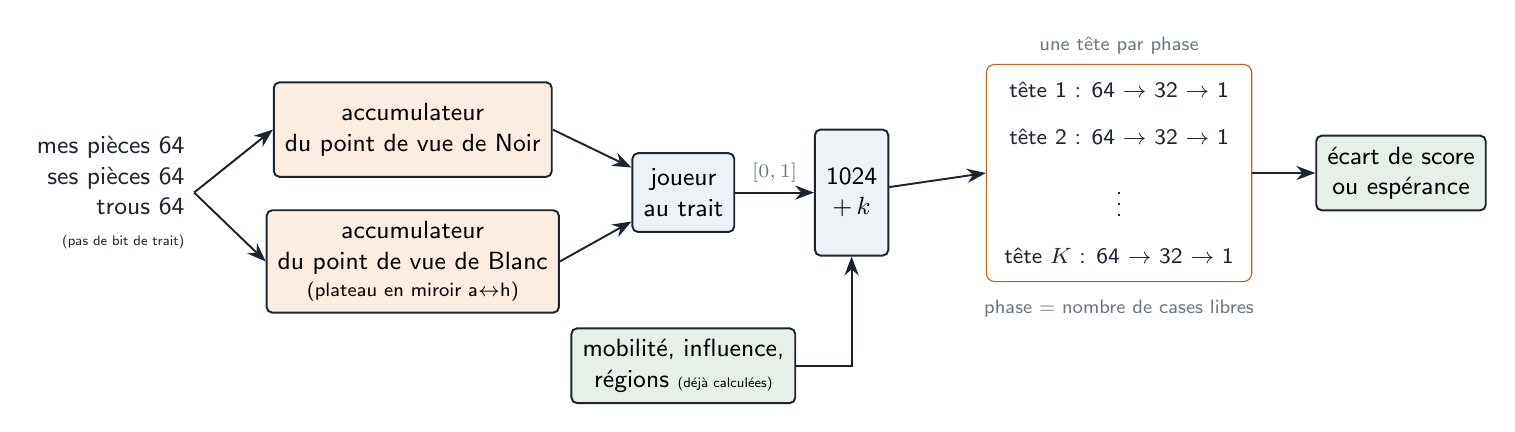
\begin{tikzpicture}[node distance=7mm]
  % two perspective accumulators
  \node[boxa,minimum width=30mm,minimum height=12mm] (am) {accumulateur\\du point de vue de Noir};
  \node[boxa,minimum width=30mm,minimum height=12mm,below=4mm of am] (aw) {accumulateur\\du point de vue de Blanc\\[-1pt]\scriptsize (plateau en miroir a$\leftrightarrow$h)};
  \node[plain,left=10mm of am,yshift=-8mm,align=right] (in) {mes pièces 64\\ses pièces 64\\trous 64\\\tiny (pas de bit de trait)};
  \draw[ar] (in.east) -- (am.west);
  \draw[ar] (in.east) -- (aw.west);
  % select by side to move
  \node[box,right=10mm of am,yshift=-8mm,minimum height=10mm] (sel) {joueur\\au trait};
  \draw[ar] (am.east) -- (sel);
  \draw[ar] (aw.east) -- (sel);
  % side features
  \node[boxb,below=12mm of sel,minimum width=28mm] (side) {mobilité, influence,\\régions \tiny (déjà calculées)};
  % concat
  \node[box,right=10mm of sel,minimum height=16mm] (cat) {1024\\$+\,k$};
  \draw[ar] (sel) -- node[tiny,above]{$[0,1]$} (cat);
  \draw[ar] (side.east) -| (cat.south);
  % buckets
  \node[plain,right=14mm of cat,yshift=13mm] (b1) {\footnotesize tête 1 : 64 $\to$ 32 $\to$ 1};
  \node[plain,below=1.5mm of b1] (b2) {\footnotesize tête 2 : 64 $\to$ 32 $\to$ 1};
  \node[plain,below=1.5mm of b2] (b3) {\footnotesize $\vdots$};
  \node[plain,below=1.5mm of b3] (b4) {\footnotesize tête $K$ : 64 $\to$ 32 $\to$ 1};
  \node[fit=(b1)(b4),draw=accent2,rounded corners=3pt,inner sep=3pt,label={[tiny]above:une tête par phase}] (heads) {};
  \draw[ar] (cat) -- (heads.west);
  \node[tiny,below=1mm of heads] {phase = nombre de cases libres};
  \node[boxb,right=8mm of heads] (v) {écart de score\\ou espérance};
  \draw[ar] (heads) -- (v);
\end{tikzpicture}
\end{document}
